%modivation.tex
\section{Motivation}

\begin{center}
  \begin{figure}[htbp]
     \begin{center}
       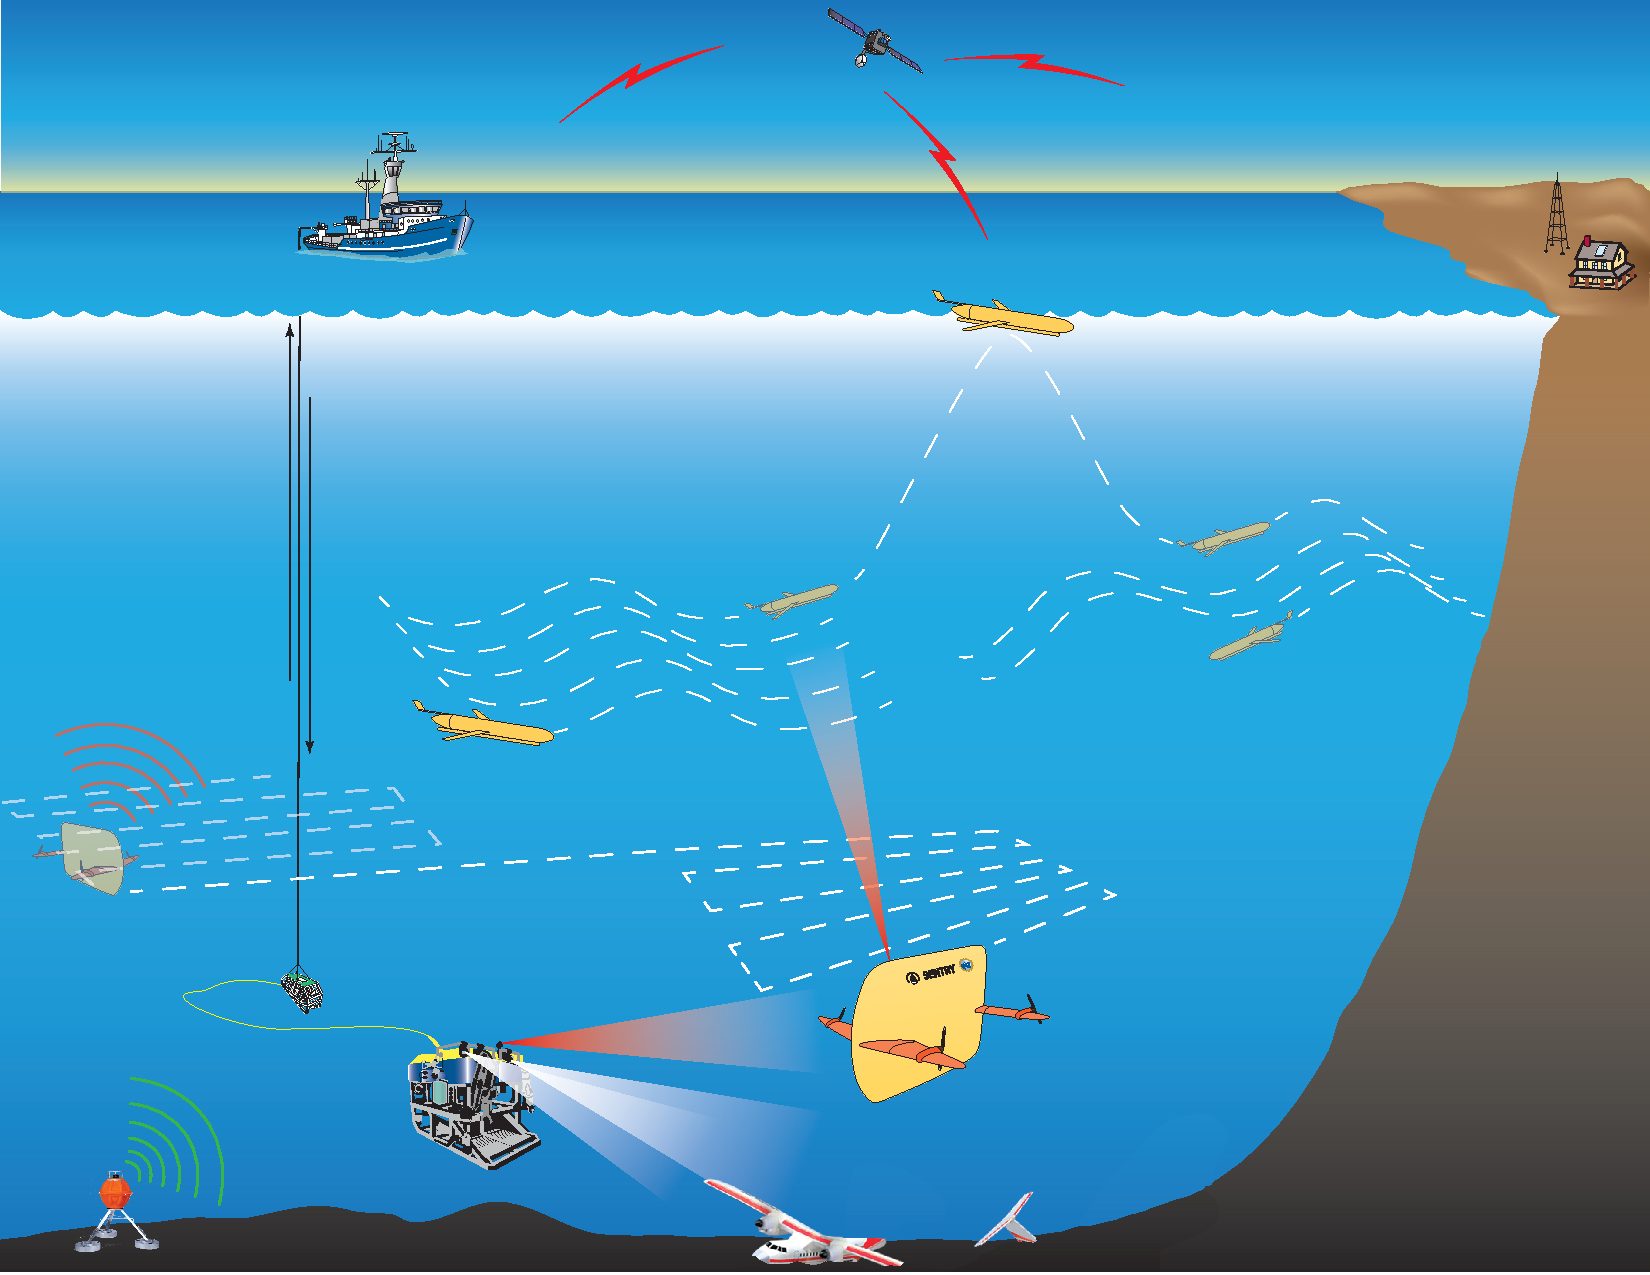
\includegraphics[width=\textwidth]{./pres/images/Adaptive4}
       \caption{Recent advances in \acf{UV} systems have enabled
         scientists and engineers to consider complex, multifaceted
         \ac{UV} missions previously thought impractical or
         impossible.  These new missions include \ac{UV} teams for
         environmental monitoring, such as the team of 5 gliders
         shown; ship-based or on-shore operator monitoring and
         re-tasking of \acp{UV}, such as the re-tasking of the
         \ac{AUV} Sentry shown; and deployment of \acp{UV} in delicate
         or dynamic environments, such as the \ac{ROV} Jason operating
         near the plane wreck shown.  {\it Improved state estimation}
         algorithms can increase navigation accuracy and lower the
         cost of \acs{UV} teams.  {\it Improved parameter
           identification} algorithms enable remote operators to
         remotely diagnose failures and use forward simulation for
         in-situ mission re-planning for \acp{UV} similar to Sentry.
         {\it Improved control} algorithms enable increased precision
         of delicate or dynamic 6-\acs{DOF} operation for \acp{ROV}
         such as Jason.  Image credit: Paul Oberlander, WHOI. }
\label{chIntro.fig.UVadaptive}
     \end{center}
  \end{figure}
\end{center}


Salt water covers over 70 \% of the surface of the earth.  
%
The world's oceans and seas to exert a huge influence on
global weather patterns, cover the longest mountain range in the
world, span 98\% of the earth's inhabitable volume, and contain
several millennia of ship wrecks.
%
Recent advances in \acf{UV} capabilities have enabled climatologists,
geologists, biologists, and archaeologists to consider addressing
research topics previously thought impractical or impossible (see
Figure \ref{chIntro.fig.UVadaptive} for examples).
%
The goal of this Thesis is to enable better utilization of these
capabilities through the development of novel algorithms for state
estimation, parameter identification, and control.
%
To this end, each type of algorithm presented herein has its own
motivating applications:
%
\begin{itemize}
%
\item {\bf State Estimation:}
%
New state estimation algorithms have the potential to improve \ac{UV}
navigation for a wide range of applications.
%
\acp{UV} operate in an environment with available sensing modalities
different from terrestrial, aerial, and on-orbit systems.
%
One consequence of these \ac{UV} specific conditions is a reliance on
dead-reckoning algorithms for translational position estimates
during 6-dimensional maneuvers.
%
It is plausible that state estimation algorithms which leverage the
group structure rigid-body motion can increase navigation
accuracy during \ac{UV} operation.
%
Such state estimation algorithms have the potential to enable \ac{UV}
navigation with different sensor suites than currently required.
%a subset of the sensor signals currently required.
%
\item {\bf Parameter Identification:} 
%
Knowledge of \ac{UV} plant parameters enable utilization of
forward simulation and other model-based algorithms for a wide range
of oceanographic research deployments.
%
The most commonly employed plant models for underwater vehicles are
finite dimensional lumped-parameter approximate models with
vehicle-specific plant parameter terms including mass and added mass
parameters; quadratic drag parameters; and gravity and buoyancy
parameters.  
%
For real-world vehicles it is impossible to compute these
plant parameters analytically, thus the plant parameters must be
identified experimentally.
%
Most previous studies of non-adaptive plant parameter identification
employ off-line conventional least-square methods requiring
instrumentation of the vehicle attitude; linear and angular velocity;
linear and angular acceleration; and applied force and moment.
%
Since \acp{UV} are often not instrumented to measure angular
acceleration, adaptive methods may provide model parameter estimates
that could not be obtained by other standard methods, such as
conventional least squares.
%
Previous adaptive parameter identification methods have focused on
model-based adaptive tracking controllers; however these approaches
are not applicable when the plant is either uncontrolled, under
open-loop control, or using any control law other than a specific
adaptive tracking controller.
%
Such conditions frequently occur on oceanographic research \ac{UV}.
%
With commercially available vehicles, often the user can not replace
the controller provided by the vehicle's manufacturer with an adaptive
tracking control algorithm.
%
Vehicle designers frequently utilize \ac{UV} passive stability of
pitch and roll in the design of under-actuated vehicles.
%
Adaptive tracking controllers assume actuation in all
degrees-of-freedom, making adaptive tracking control inapplicable for
either control or model identification of under-actuated vehicles.
%
Adaptive identification algorithms do not require simultaneous
reference trajectory-tracking control, nor do they require
instrumentation of linear acceleration or angular acceleration.

\item{\bf Trajectory-Tracking:} 
%
Many of the missions recently enabled by advances in \ac{UV}
technology, such as seafloor surveying and environmental
monitoring, depend on tracking a specified trajectory as closely as
possible.
%
To facilitate these missions, novel \ac{UV} control algorithms are
required to provide improved trajectory-tracking precision.
%
Previous studies have shown experimentally that \acl{MBC} can provide
significant performance gains over \acl{PDC}\cite{martinID_ICRA13,
smallwood2004JOE}. 
%
For most \acp{UV} the drag parameters and mass parameters (which include
both the characteristics of the vehicle's mass and those of the
ambient fluid surrounding the vehicle) can not be computed
analytically.
%
Adaptive model-based control removes the need for {\it a-priori}
parameter estimates and could enable accurate long duration trajectory
tracking through continuous model retuning.
%
\end{itemize}




% A second 

%  is to add to the toolbox of algorithms
% available for this research.
% %

% operationally relevent trajectories; 


% better 
% %


% state estimates

% This thesis 

% State observers
% %
% Picture of Jason
% %
% Picture of Nereus
% %

% low cost sensors - does not apply

% something about applying techniques from geometry control, 



% We are developing
% adaptive modeling techniques which model drag, buoyancy, inertia and
% hydrodynamic forces.  These methods 'learn' the correct parameter
% values either independently or as part of the control process.  We
% believe these methods will significantly improve UUV effectiveness for
% scientific research.


% model identification can aid 

% The Goal of this thesis is 

% use recent advances in geometric control, robotics, and ____ to develop algorithms 